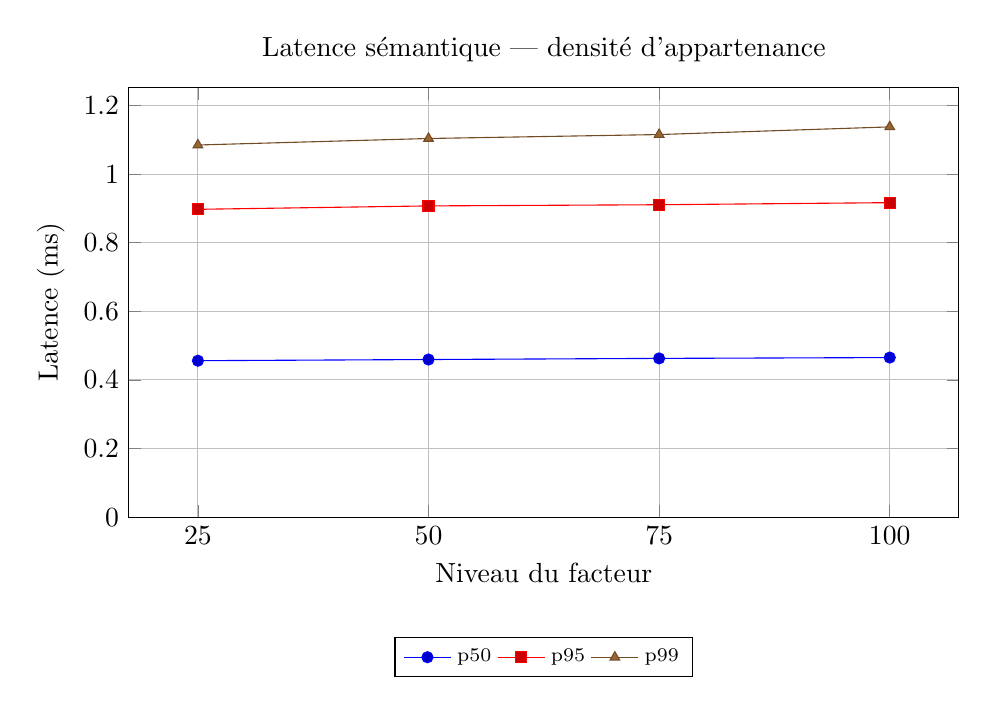
\begin{tikzpicture}
\begin{axis}[width=\linewidth,
height=0.58\linewidth,
title={Latence sémantique — densité d'appartenance},
xlabel={Niveau du facteur},
ylabel={Latence (ms)},
grid=major,
legend style={font=\scriptsize,at={(0.5,-0.28)},anchor=north,legend columns=3},
xtick={25.0,50.0,75.0,100.0},
ymin=0]
\addplot+[mark=*] coordinates {(25.0,0.4560535) (50.0,0.4595035) (75.0,0.462777) (100.0,0.46519)};
\addlegendentry{p50}
\addplot+[mark=square*] coordinates {(25.0,0.8974601) (50.0,0.9074034) (75.0,0.9108173) (100.0,0.9169272)};
\addlegendentry{p95}
\addplot+[mark=triangle*] coordinates {(25.0,1.0849937) (50.0,1.10397349) (75.0,1.11547759) (100.0,1.13779353)};
\addlegendentry{p99}
\end{axis}
\end{tikzpicture}
